\section{Method}
\label{sec:methods}


\subsection{Optimization Target Formulation}
\label{sec:problem_formulation}

We start by focusing on a hidden layer matrix $\mW\in\mathbb{R}^{d_{\text{out}}\times d_{\text{in}}}$. To satisfy the spectral $\boldsymbol{\mu}$P scaling condition in~\cref{sec:bg_mup}, we set the spectral scale to target radius $R$:
\begin{equation}
\label{eq:radius_def}
R = \Theta\left(\sqrt{d_{\text{out}}/d_{\text{in}}}\right).
\end{equation}
Following metrized deep learning (\cref{sec:bg_mdl}), we define the unit update $\mPhi$ as the solution to a constrained optimization problem:


\begin{mdframed}[style=MyBoxStyle2, frametitle={Formulation: Steepest Descent on the Spectral Sphere}, nobreak=true]

We perform \textbf{steepest descent} under the \textbf{spectral norm}, constraining both the \textbf{weights} and the \textbf{updates} to a spectral sphere of radius $R$. Specifically, we parameterize the update step as $\Delta \mW = \eta R \mPhi$, where $\eta$ is the base learning rate. The update direction $\mPhi$ is the solution to:
\begin{equation}
\label{eq:opt_problem}
\begin{aligned}
\max_{\mPhi}\quad & \langle \mG, \mPhi \rangle \\
\text{s.t.}\quad & \|\mPhi\|_2 = 1, \\
                 & \|\mW - \eta R \mPhi\|_2 = \|\mW\|_2 = R.
\end{aligned}
\end{equation}
\end{mdframed}

\subsection{First-Order Tangent Space Constraint}
\label{sec:tangent_linearization}

Assisted by the uniqueness of the top singular value\footnote{Numerical coincidence of singular values is a measure-zero event for random matrices~\citep{tao2014randommatricessimplespectrum}. Quantitatively, it occurs with probability at most $\exp(-c\max(d_{\mathrm{in}},d_{\mathrm{out}}))$~\citep{han2025repeatedsingularvaluesrandom}.}, the spectral norm $\|\mW\|_2$ is differentiable with gradient $\mTheta := \nabla_{\mW}\|\mW\|_2 = \vu_1 \vv_1^\top$, where $(\vu_1, \vv_1)$ are the principal left and right singular vectors~\citep{watson1992characterization}.
We consider a first-order Taylor Expansion of the spectral norm around $\mW$:
\begin{equation}
\label{eq:taylor_spectral}
\|\mW - \eta R \mPhi\|_2 = \|\mW\|_2 - \eta R \langle \mTheta, \mPhi \rangle + \mathcal{O}(\eta^2 R^2 \|\mPhi\|_2^2).
\end{equation}
To enforce the invariance condition $\|\mW - \eta R \mPhi\|_2 = \|\mW\|_2$, the first-order term must vanish, which implies the tangent constraint:$\langle \mTheta, \mPhi \rangle = 0$.
\cref{eq:opt_problem} thus reduces to
\begin{equation}
\label{eq:linearized_opt}
\max_{\mPhi}\ \langle \mG,\mPhi\rangle
\quad \text{s.t.}\quad
\|\mPhi\|_2\ = 1,\ \ \langle \mTheta,\mPhi\rangle = 0.
eq\end{equation}
We then introduce a \emph{Lagrange multiplier} \(\lambda\) and maximize \emph{Lagrangian}  \( \mathcal{L}(\mPhi; \lambda) =  \langle \mG+\lambda\mTheta,\mPhi\rangle\) under constraint \(\|\mPhi\|_2=1\). The analytical solution and numerical method are summarized below.


\begin{mdframed}[style=MyBoxStyle2, frametitle={Solution: Tangent Space Update via $\lambda$-Search}]
    For a fixed $\lambda$, the steepest descent direction is (proof in~\cref{app:dual})
    \begin{equation}
        \label{eq:optimal_phi}
        \mPhi^\star(\lambda) = \operatorname{msign}(\mG + \lambda \mTheta),
    \end{equation}
    where $\lambda^\star$ is the unique root of the constraint function
    \begin{equation}
        h(\lambda) := \langle \mTheta, \operatorname{msign}(\mG + \lambda \mTheta) \rangle, \quad h(\lambda^\star) = 0.
    \end{equation}

    \textbf{Theoretical Properties} (proof in~\cref{app:localization}, visualized in~\cref{fig:f_lambda_numeric}):
    \begin{enumerate}[label=\roman*), leftmargin=1.5em, itemsep=2pt, topsep=2pt]
        \item \textbf{Monotonicity:} The function $h(\lambda)$ is monotonically non-decreasing and transitions from $-1$ to $+1$ as $\lambda$ varies from $-\infty$ to $+\infty$.
        \item \textbf{Root Localization:} The solution $\lambda^\star$ is strictly bounded within the interval $[-2\|\mG\|_*,\, 2\|\mG\|_*]$, providing a finite search space~\footnote{Nuclear norm $\|\!\cdot\!\|_*$ is the sum of singular values.}.
    \end{enumerate}

    \vspace{4pt}
    \textbf{Numerical Algorithm} (overhead analysis in~\cref{sec:system}):

    Given the monotonic nature of $h(\lambda)$, we locate $\lambda^\star$ efficiently:
    \begin{itemize}[leftmargin=1.5em, label=$\triangleright$, itemsep=2pt, topsep=2pt]
        \item \textbf{Bracketing:} Leveraging monotonicity, we start from $\lambda = 0$ and exponentially expand the search bracket in the opposite direction of the sign of $h(0)$ until the root is enclosed.
        \item \textbf{Bisection:} We isolate $\lambda^\star$ via standard bisection within the bracketed interval.
    \end{itemize}
\end{mdframed}
\begin{figure}[ht]
    \centering
    \begin{subfigure}
        {0.45\linewidth}
        \centering
        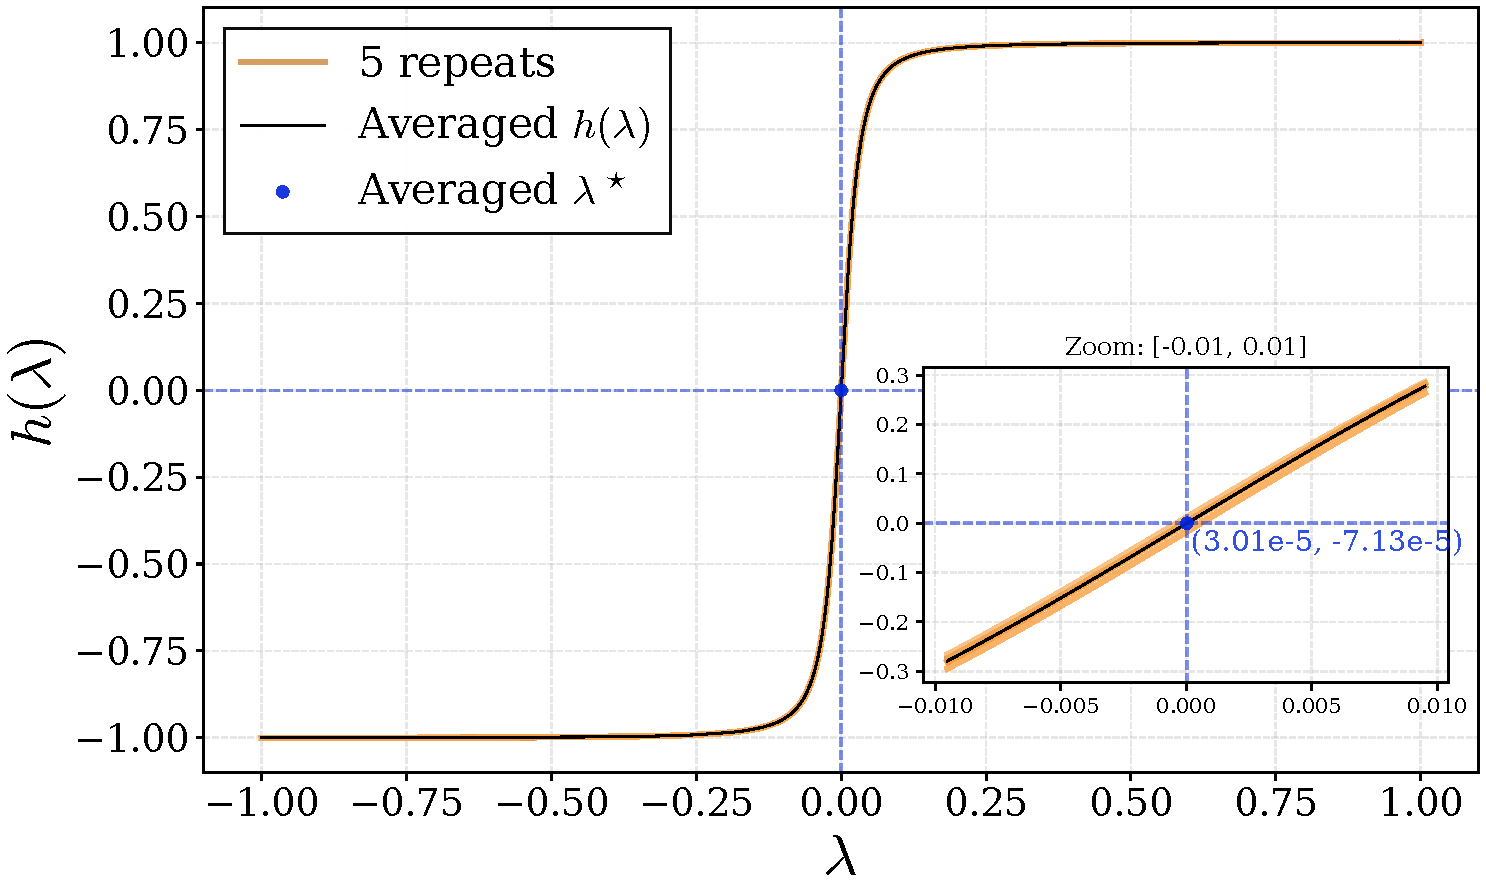
\includegraphics[width=\linewidth]{figures/appendix/h_lambda_1024x3072_mean0.0_std0.02_n5.pdf}
        \caption{$1024 \times 3072$ matrix}
    \end{subfigure}
    \hfill
    \begin{subfigure}
        {0.45\linewidth}
        \centering
        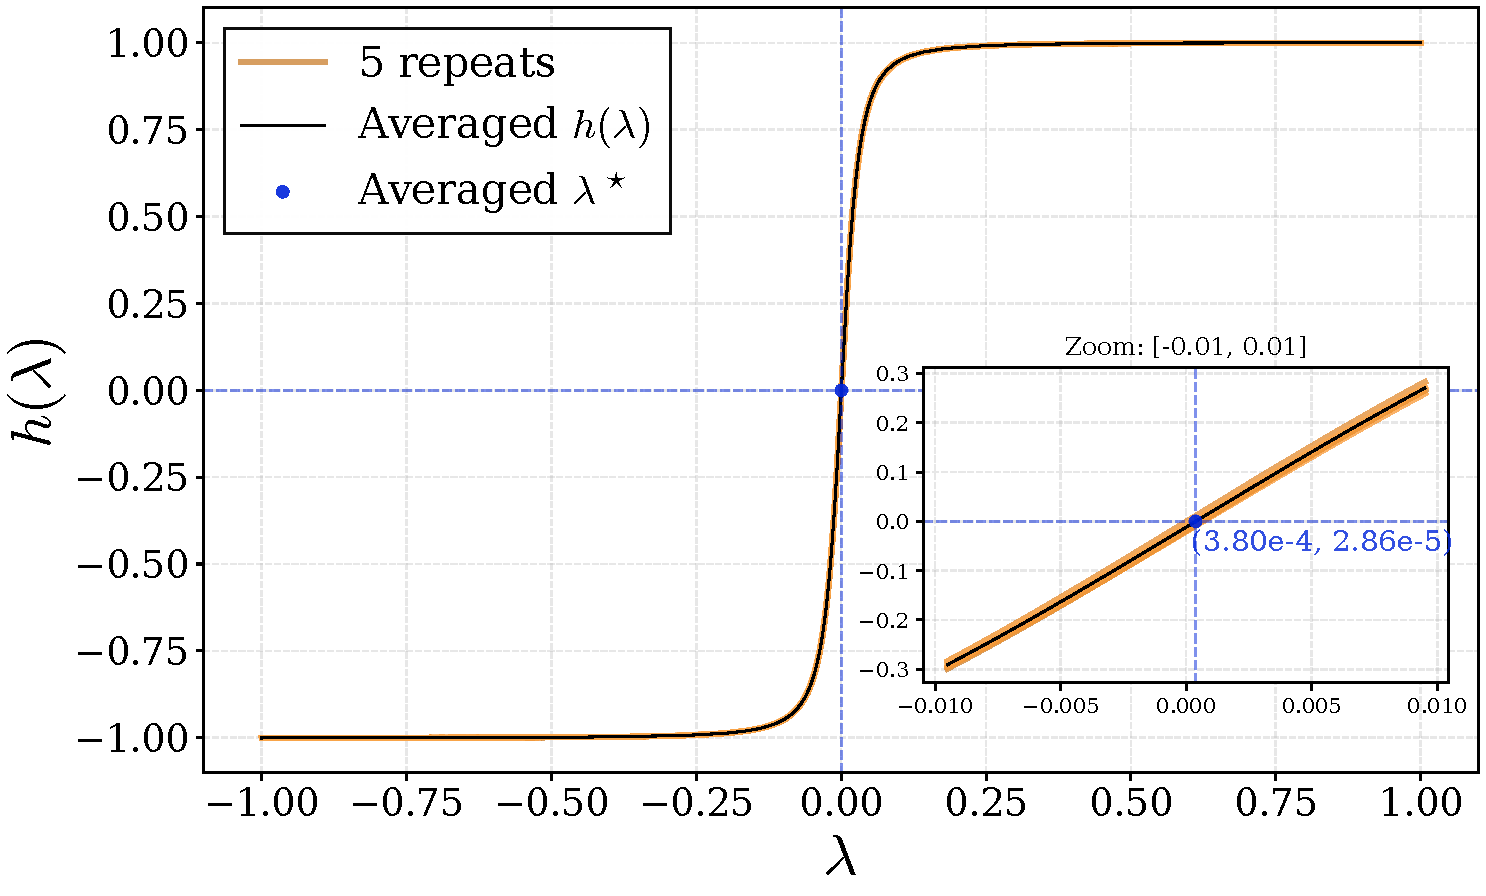
\includegraphics[width=\linewidth]{figures/appendix/h_lambda_4096x1024_mean0.0_std0.02_n5.pdf}
        \caption{$4096 \times 1024$ matrix}
    \end{subfigure}
    \caption{\textbf{Empirical curves of} $h(\lambda) = \langle \mTheta, \operatorname{msign}(\mG + \lambda \mTheta) \rangle$ \textbf{for random matrices}. $h(\lambda)$ is monotonic non-decreasing in $\lambda$, and its root $\lambda^\star$ lies close to zero (proof in~\cref{app:localization}). Here, each curve is obtained by averaging over 5 repeats, and each matrix is initialized from $\mathcal{N}(0,0.02^2)$.}
    \label{fig:f_lambda_numeric}
\end{figure}


\subsection{Second-Order Manifold Constraint}
\label{sec:retraction}
Note that the remainder $\mathcal{O}(\eta^2 R^2 \|\mPhi\|_2^2)$  in~\cref{eq:taylor_spectral} may accumulate over iterations, causing gradual drift off the spectral sphere. To enforce the exact constraint $\|\mW\|_2 = R$ throughout training, we apply a retraction step that projects the weights back onto the manifold:
\begin{equation}
\label{eq:retraction_map}
\mW
\gets
\mW\cdot \frac{R}{\|\mW\|_2}.
\end{equation}
While the retraction is conceptually a post-update projection, we implement it as a pre-update correction for efficiency, which is operationally equivalent. This reordering allows us to invoke the computationally expensive Power Iteration only once per step, reusing the resulting singular triplet for both the manifold retraction and the tangent projector $\mTheta$ (Lines 6--9 in~\cref{alg:sso}).


The retraction strictly constrains $\|\mW\|_2=R$, which via~\cref{eq:weight_bound}, automatically bounds the weight magnitudes. As a result, weight decay, which is primarily introduced to limit the weight scale, becomes redundant. We therefore \textbf{eliminate weight decay}
in hidden 2D weights\footnote{We still apply weight decay to params like \texttt{Embedding} for possible scaling stability, although our ablations on 1.7B model suggest that disabling weight decay may actually be slightly better.}, removing a sensitive hyperparameter from training. More details can be found in~\cref{app:wd_retract}.
\begin{equation}
    \label{eq:weight_bound}
    \|\mW\|_F \le \sqrt{rank(\mW)}\,\|\mW\|_2
    \le \sqrt{\min(d_{\text{out}},d_{\text{in}})}\,R .
\end{equation}

%\subsection{Algorithm Summary \& Interpretation}
\subsection{Overall Algorithm \& Interpretation}
\begin{algorithm}[ht]
    \caption{Spectral Sphere Optimizer (SSO)}
    \label{alg:sso}
    \begin{algorithmic}[1]
        \Require
            Initial 2D weights $\mW_0 \in \mathbb{R}^{d_{\text{out}} \times d_{\text{in}}}$,
            spectral $\boldsymbol{\mu}$P scaler $R = \sqrt{d_{\text{out}}/d_{\text{in}}}$,
            learning rate $\eta$,
            momentum coefficient $\beta$,
            precision tolerance $\epsilon$
        \State \textbf{Initialize:} $\mW_0 \gets R \cdot \mW_0 / \|\mW_0\|_2$, $\mM_0 \gets 0$

        \For{$t = 0, 1, \dots$}
            \State $\mG_t \gets \nabla_\mW \mathcal{L}(\mW_t)$
            \State $\mM_t \gets \beta \mM_t + (1-\beta) \mG_t$
            \State $\widehat{\mM}_t \gets \mM_t / \|\mM_t\|_F$ \hfill \Comment{Normalize for Numerical Stability}

            \Statex \textcolor{gray}{\textbf{\itshape // 1. Spectral Geometry Analysis}}
            \State $(\evsigma_{t}, \vu_{t}, \vv_{t}) \gets \mathrm{PowerIteration}(\mW_{t})$ \hfill \Comment{Top Singular Value \& Vectors}
            \State $\mTheta_t \gets \vu_t \vv_t^\top$ \hfill \Comment{Tangent Space Projector}

            \Statex \textcolor{gray}{\textbf{\itshape // 2. Retraction to Spectral Sphere}}
            \State $\mW_t \gets \mW_t \cdot R / \evsigma_{t}$

            \Statex \textcolor{gray}{\textbf{\itshape // 3. Steepest Descent Lagrange Solver}}
            \State Define $h(\lambda) \coloneqq \langle \mTheta_t, \operatorname{msign}(\widehat{\mM}_t + \lambda \mTheta_t) \rangle$
            \State $\lambda_t^* \gets \mathrm{Bisection}(h, \text{tolerance}=\epsilon)$ \hfill \Comment{Find root of $h(\lambda)=0$}

            \Statex \textcolor{gray}{\textbf{\itshape // 4. $\boldsymbol{\mu}$P-Scaled Update}}
            \State $\mPhi_t \gets \operatorname{msign}(\widehat{\mM}_t + \lambda_t^* \mTheta_t)$
            \State $\mW_{t+1} \gets \mW_t - \eta \cdot R \cdot \mPhi_t$ \hfill \Comment{$\boldsymbol{\mu}$P Style Update}
        \EndFor
    \end{algorithmic}
\end{algorithm}

In this paper, we set AdamW and Muon as baselines. Additionally, we introduce MuonSphere, a variant similar to Scion~\citep{pethick2025trainingdeeplearningmodels}\footnote{Unlike Scion, which applies ColNorm$\to$Spectral$\to$Sign ($l_{\infty}$) norm chain throughout the network, MuonSphere retains Sign$\to$Spectral$\to$Sign norm scheme. We find ColNorm input hurts performance.}, which can be viewed as Spectral Sphere with $\lambda=0$. While Spectral Sphere follows a steepest-descent approach, MuonSphere simply normalizes 2D hidden weights onto the spectral sphere before each update. \cref{fig:sketch} provides a sketch of the latter three spectral-preconditioned optimizers' update.
\begin{figure}[ht]
    \centering
    %\vspace{-1em}
    % \begin{overpic}[scale=0.2]{figures/method/sso20.pdf}
    %     \put(68,3){\includegraphics[width=2.5cm]{figures/method/denotes.png}}
    % \end{overpic}
    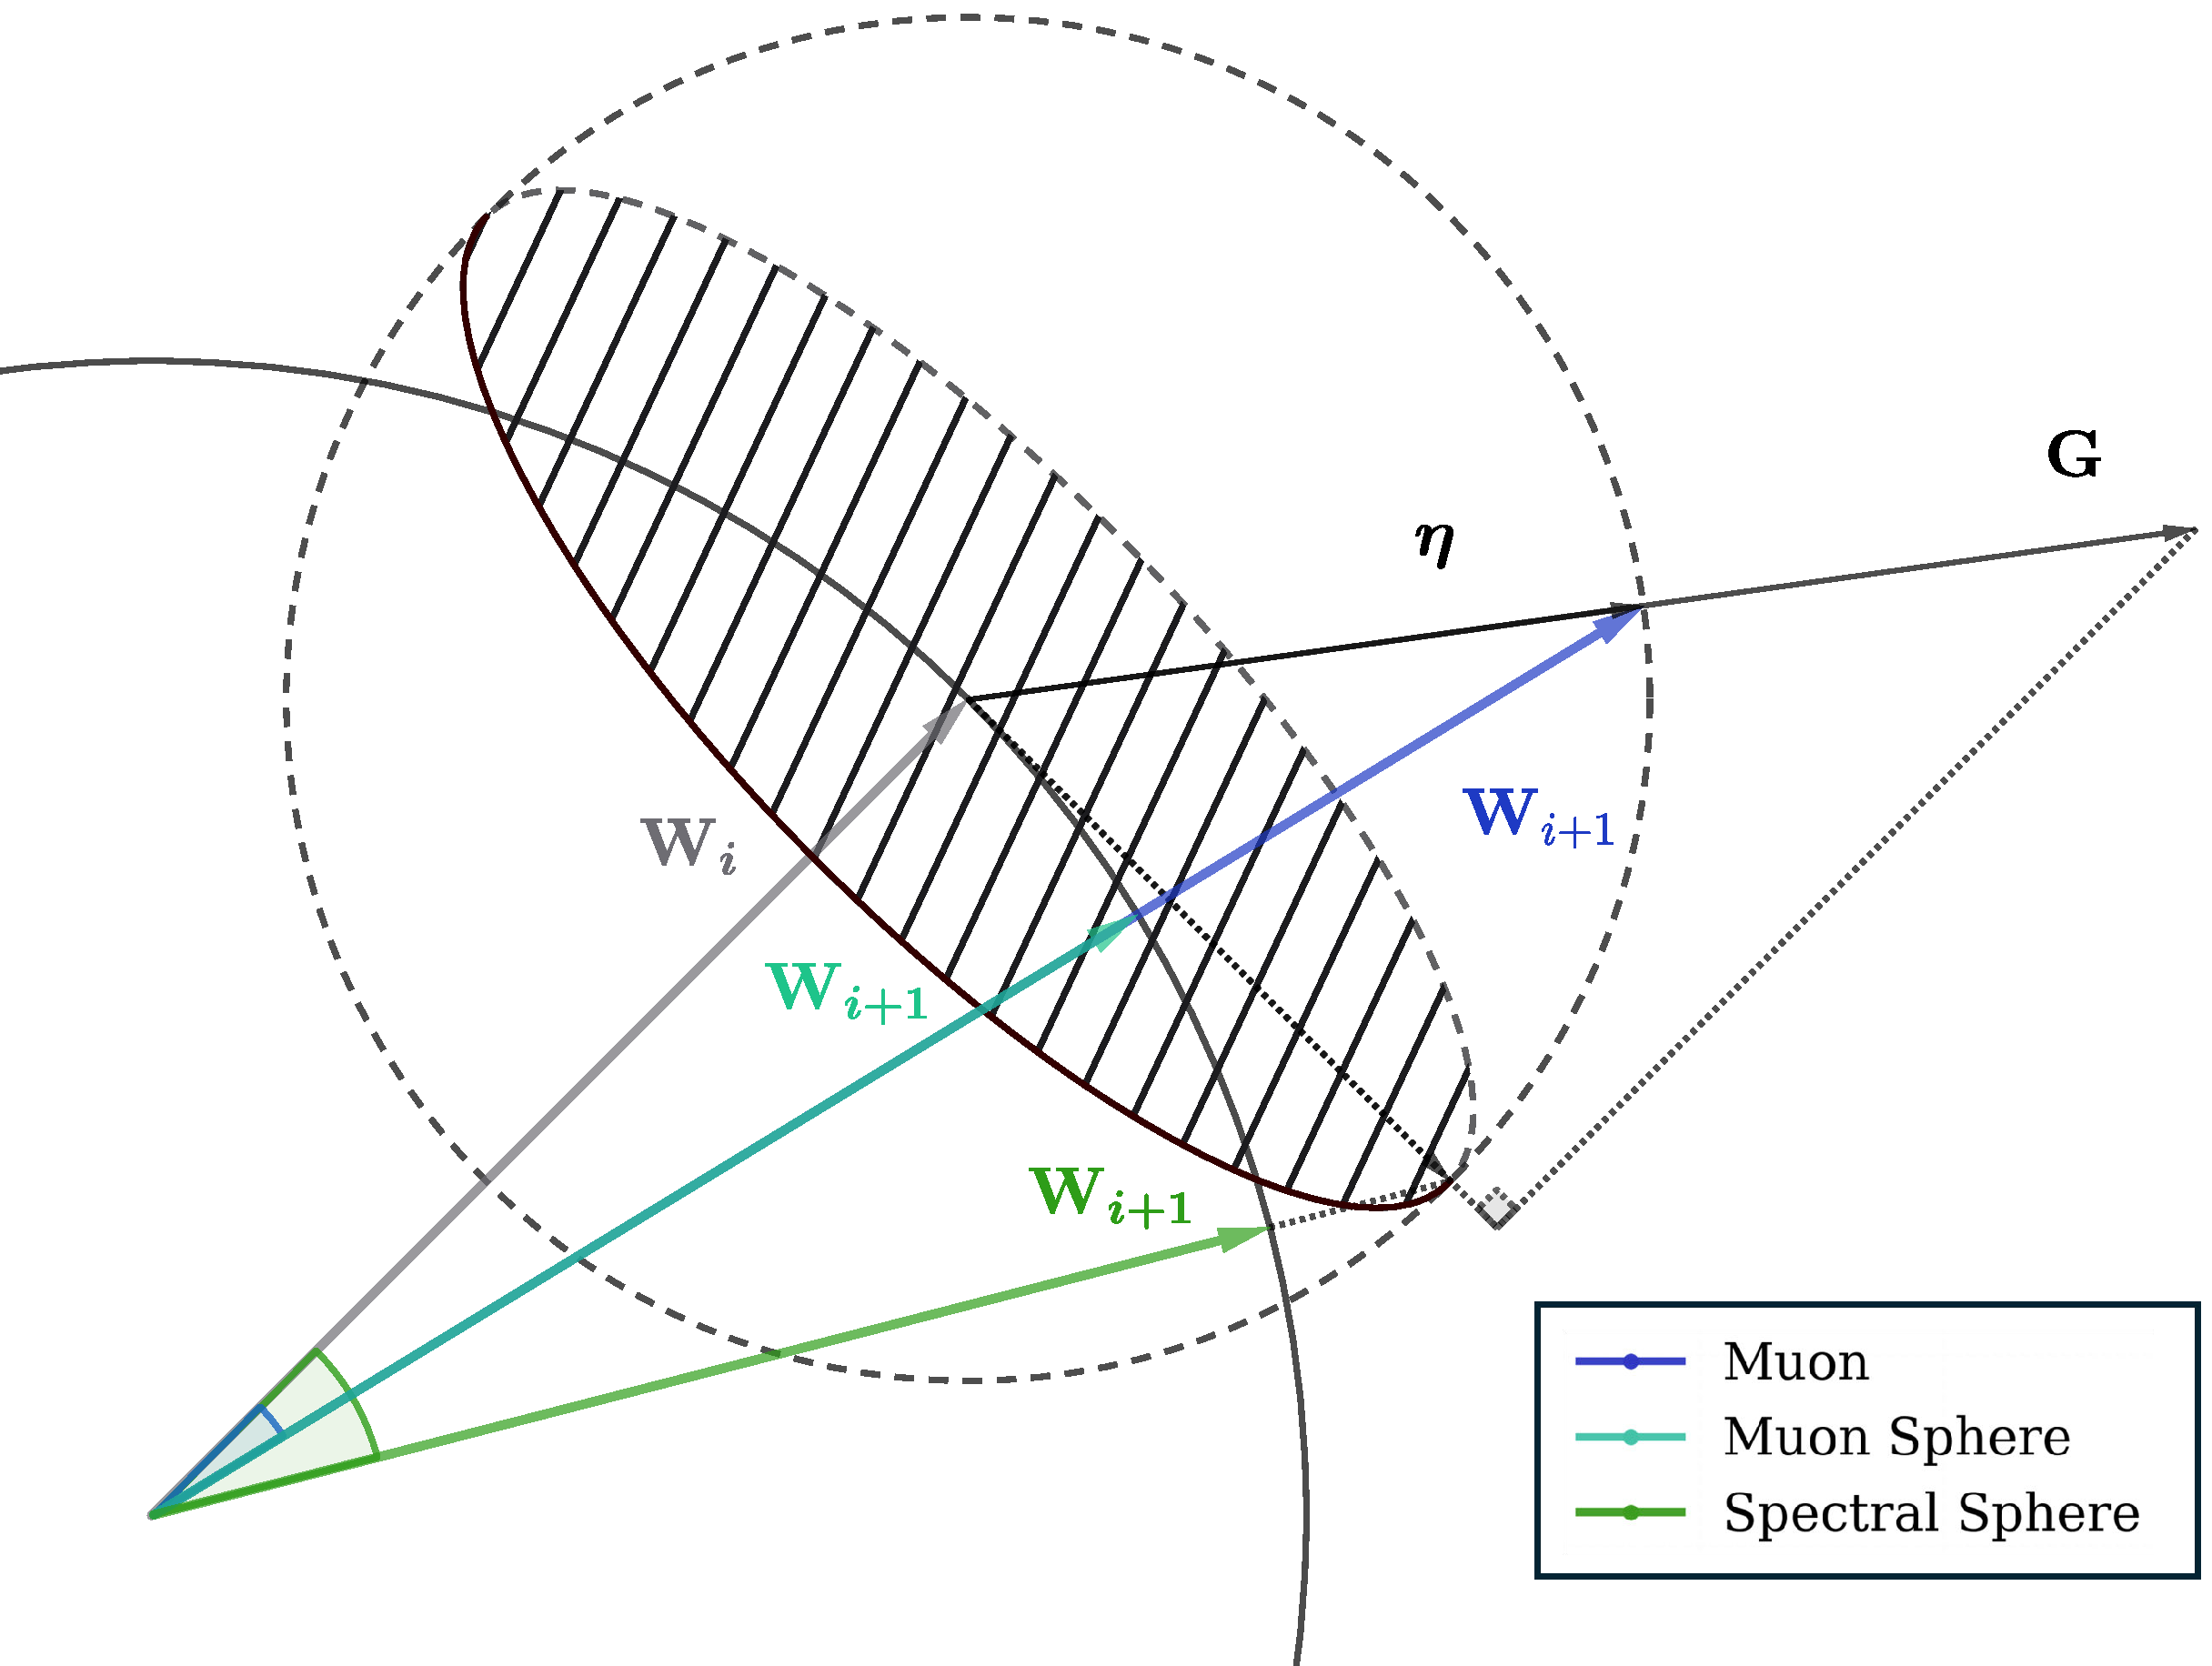
\includegraphics[scale=0.2]{figures/method/sso.pdf}
    \caption{\textbf{Geometry of Steepest Descent Update Directions.}
    The left solid arc denotes the $\mW$ sphere, while the right dotted arc denotes the $\Delta \mW$ sphere (unit $\mPhi$ scaled by $\eta$).
    The shaded region represents the feasible set within the \emph{tangent space} of the $\mW$ sphere at step $\mW_i$.
    Under weight constraint, projecting $\mG$ onto the tangent space (\textcolor{SpectralSphereColor}{Spectral Sphere}) yields the largest update angle.}
    \label{fig:sketch}
\end{figure}
